\chapter[Nível de Time]{Nível de Time}

\section{Planejamento da 1ª Iteração}

No planejamento da primeira iteração foram alocadas as seguintes histórias:

\begin{figure}[!htb]
\centering
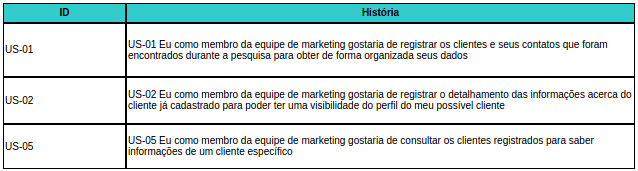
\includegraphics[scale=0.8]{figuras/backlog_iteracao.png}
\caption{\textit{Backlog} da primeira iteração}
\label{fig:backlog}
\end{figure}

\section{Especificação das Histórias}

\subsection{Iteração 1}

\textbf{US-01} Eu como membro da equipe de marketing gostaria de registrar os clientes e seus contatos que foram encontrados durante a pesquisa para obter de forma organizada seus dados.

\begin{itemize}
 \item Critérios de aceitação:
\subitem O registro deve conter os seguintes campos: Nome, Telefone, Email, Logradouro, CEP, cidade de localização, site e Informações adicionais.
\subitem Um registro só dever ser salvo quando pelo menos os campos de Nome e algum dos contatos (telefone, email, endereço) estiver corretamente preenchido.
\subitem Pode ocorrer o registro de mais de um telefone.
\subitem Pode ocorrer o registro de mais de um email.
\subitem O cliente deve ser identificado através de um código gerado automaticamente.

\item Tarefas:
\subitem Criar formulário de registro com botão para salvar os dados.
\subitem Criar validação dos campos de Nome e dos contatos (telefone, email, endereço) seguindo a lógica definida no critério de aceitação.
\subitem Criar evento no botão que permite armazenar o registro no banco de dados.
\end{itemize}

\textbf{US-02} Eu como membro da equipe de marketing gostaria de registrar o detalhamento das informações acerca do cliente já cadastrado para poder ter uma visibilidade do perfil do meu possível cliente.

\begin{itemize}
 \item Critérios de aceitação:
\subitem O registro deve conter os seguintes campos: Tamanho da empresa, Área de atuação, CNPJ e representante da empresa contatada.
\subitem O tamanho da empresa pode ser de pequeno, médio ou grande porte.
\subitem O preenchimento desse registro não é obrigatório.

\item Tarefas:
\subitem Criar interface com formulário para inserção dos dados com opção de salvar os dados.
\subitem Implementar evento que é disparado quando o botão de salvar é clicado.
\subitem Implementar método que armazena os dados no banco de dados.


\end{itemize}

\textbf{US-05} Eu como membro da equipe de marketing gostaria de consultar os clientes registrados para saber informações de um cliente específico.

\begin{itemize} 
\item Critérios de aceitação:
\subitem A consulta deve ser em uma lista de todos os clientes registrados.
\subitem A consulta deve mostrar as informações completas do cliente (básicas e detalhadas) com os campos que estão preenchidos.
\subitem A consulta pode ser realizada por nome da empresa, área de atuação, por CNPJ e por tamanho.
\subitem A consulta por área de atuação pode ser combinada com a consulta por tamanho e vice-versa.
\subitem A partir da consulta realizada, o usuário pode ser redirecionado à página de visualização do cliente.

\item Tarefas:
\subitem Criar uma lista com todos os clientes cadastrados.
\subitem Criar página para mais fácil visualização e edição de clientes registrados.
\subitem Criar \textit{dropdown} com os termos “pequena, média e grande”.
\subitem Abstrair lógica para dupla filtragem CNPJ-tamanho.
\end{itemize}


Algumas histórias previstas na Iteração 2 também foram especificadas.
\section{Iteração 2}

\textbf{US-03} Eu como membro da equipe de \textit{marketing} gostaria de editar os clientes e seus contatos que foram encontrados durante a pesquisa para manter suas informações atualizadas.

\begin{itemize}
  \item Critérios de aceitação:
\subitem O ID é o único campo que não pode ser editado.
\subitem Os campos de detalhamento não podem ser editados.
 
\end{itemize}


\textbf{US-04} Eu como membro da equipe de \textit{marketing} gostaria de editar o detalhamento das informações acerca do cliente já cadastrado para manter o registro atualizado.
\begin{itemize}
\item Critérios de aceitação:
\subitem O ID é o único campo que não pode ser editado.
\subitem Os campos básicos não podem ser editados.

\end{itemize}




